\documentclass[journal,12pt,onecolumn]{IEEEtran}
\usepackage{cite}
\usepackage{graphicx}
\usepackage{amsmath,amssymb,amsfonts,amsthm}
\usepackage{algorithmic}
\usepackage{graphicx}
\usepackage{textcomp}
\usepackage{xcolor}
\usepackage{txfonts}
\usepackage{listings}
\usepackage{enumitem}
\usepackage{mathtools}
\usepackage{gensymb}
\usepackage{comment}
\usepackage[breaklinks=true]{hyperref}
\usepackage{tkz-euclide} 
\usepackage{listings}
\usepackage{gvv}                                        
\usepackage[latin1]{inputenc} 
\usetikzlibrary{arrows.meta, positioning}
\usepackage{xparse}
\usepackage{color}                                            
\usepackage{array}                                            
\usepackage{longtable}                                       
\usepackage{calc}                                             
\usepackage{multirow}
\usepackage{multicol}
\usepackage{hhline}                                           
\usepackage{ifthen}                                           
\usepackage{lscape}
\usepackage{tabularx}
\usepackage{array}
\usepackage{float}
\newtheorem{theorem}{Theorem}[section]
\newtheorem{problem}{Problem}
\newtheorem{proposition}{Proposition}[section]
\newtheorem{lemma}{Lemma}[section]
\newtheorem{corollary}[theorem]{Corollary}
\newtheorem{example}{Example}[section]
\newtheorem{definition}[problem]{Definition}
\newcommand{\BEQA}{\begin{eqnarray}}
\newcommand{\EEQA}{\end{eqnarray}}
\usepackage{float}
\theoremstyle{remark}
\usepackage{circuitikz}
\usepackage{tikz}



\title{GATE 2009 GG: GEOLOGY AND GEOPHYSICS}
\author{EE25BTECH11032 -Kartik Lahoti}
\date{}

\begin{document}
\maketitle
    \begin{center}
        \subsection*{PART A: COMMON TO BOTH GEOLOGY AND GEOPHYSICS CANDIDATES}
    \end{center}
\subsubsection*{Q.1 - Q.20 carry one mark each.}

    \begin{enumerate}                                 
     \item The Gutenberg discontinuity is located at a depth of around \hfill{\hfill{\brak{\text{GATE GG 2009}}}} 
            \begin {enumerate}
                \begin{multicols}{2}
                    \item$35\,km$
                    \item$150\,km$
                    \item$2900\,km$
                    \item$5000\,km$
                \end{multicols}
            \end{enumerate}
         
    \item What is the age of the "Barail Series"? \hfill{\hfill{\brak{\text{GATE GG 2009}}}} 
            \begin {enumerate}
                \begin{multicols}{2}
                    \item Jurassic
                    \item Paleocene
                    \item Oligocene
                    \item Miocene
                \end{multicols}
            \end{enumerate}            

    \item Thermohaline circulation in the oceans is driven by \hfill{\hfill{\brak{\text{GATE GG 2009}}}} 
            \begin{enumerate}
                \item only salinity gradients
                \item both temperature and salinity gradients
                \item only temperature gradients
                \item only density difference
            \end{enumerate}
        
    \item Which one of the following minerals cannot be used as an abrasive ? \hfill{\brak{\text{GATE GG 2009}}} 
                \begin {enumerate}
                    \begin{multicols}{2}
                        \item Garnet
                        \item Corundum
                        \item Quartz
                        \item Gypsum
                    \end{multicols}
            \end{enumerate}
        
    \item Which one of the following lakes is interpreted to be of meteoritic impact origin ? \hfill{\brak{\text{GATE GG 2009}}} 
            \begin {enumerate}
                \begin{multicols}{2}
                    \item Lonar Lake
                    \item Chilika Lake
                    \item Kolleru Lake
                    \item Pulicat Lake
                \end{multicols}
            \end{enumerate}
            
    \item Which one of the following geomorphic features is \textbf{not} related to desert environments ? \hfill{\brak{\text{GATE GG 2009}}} 
            \begin {enumerate}
                \begin{multicols}{2}
                    \item yardang
                    \item bajada
                    \item hamada
                    \item esker
                \end{multicols}
            \end{enumerate}            
            
    \item Which one of the following is located closest to the Ninety-East Ridge ?  \hfill{\brak{\text{GATE GG 2009}}} 
            \begin{enumerate}
                \item Bombay High
                \item Lakshwadweep Islands
                \item Andaman And Nicobar Islands
                \item Maldives                
            \end{enumerate}
            
     \item LPG (Liquefied Petroleum Gas) consists mainly of \hfill{\brak{\text{GATE GG 2009}}}  
            \begin{enumerate}
                \item propane and butane
                \item methane and ethane
                \item methane and butane
                \item ethane and propane              
            \end{enumerate}    
            
    \item Who proposed the principle "the present is the key to the past"? \hfill{\brak{\text{GATE GG 2009}}}  
            \begin {enumerate}
                \begin{multicols}{2}
                    \item Carl von Linnaeus
                    \item James Hutton
                    \item William Smith
                    \item Alcide d'Orbigny
                \end{multicols}
            \end{enumerate}
            
    \item Of the following, which is an ore of nickel? \hfill{\brak{\text{GATE GG 2009}}} 
            \begin {enumerate}
                \begin{multicols}{2}
                    \item Pentlandite
                    \item Cinnabar
                    \item Cassiterite
                    \item Scheelite
                \end{multicols}
            \end {enumerate}
            
    \item  Over a three layered earth, comprising of top dry soil followed by saturated weathered layer and hard rock basement, a resistivity sounding experiment is performed. The obtained VES curve is \hfill{\brak{\text{GATE GG 2009}}} 
             \begin {enumerate}
                \begin{multicols}{2}
                    \item K-type  
                    \item A-type
                    \item H-type
                    \item Q-type
                \end{multicols}
            \end{enumerate}
            
    \item The logging tool for direct determination of permeability is \hfill{\brak{\text{GATE GG 2009}}} 
            \begin {enumerate}
                \begin{multicols}{2}
                    \item induction
                    \item litho-density
                    \item sonic
                    \item NMR
                \end{multicols}
            \end{enumerate}
            
    \item Which of the following parameters is uniquely resolved by residual gravity anomaly data? \hfill{\brak{\text{GATE GG 2009}}}   
            \begin{enumerate}
                \item lateral density contrast 
                \item excess/deficit mass
                \item absolute density
                \item geometric dimensions of geophysical model                 
            \end{enumerate}
            
    \item Crude oil density, in degree API (American Petroleum Institute), is a measure of viscosity. The value of $10$ API is of \hfill{\brak{\text{GATE GG 2009}}}  
            \begin {enumerate}
                \begin{multicols}{2}
                    \item water
                    \item heavy crude
                    \item average crude
                    \item light crude
                \end{multicols}
            \end{enumerate}
            
    \item For perfectly conducting medium, skin depth $\brak{m}$ is \hfill{\brak{\text{GATE GG 2009}}} 
            \begin {enumerate}
                \begin{multicols}{2}
                    \item $10^5$
                    \item $100$
                    \item $10$
                    \item $0$
                \end{multicols}
            \end{enumerate}
            
    \item If a planet revolves around the Sun with a period of $8$ years, then its distance from the Sun would be (in terms of distance between Earth and Sun) \hfill{\brak{\text{GATE GG 2009}}} 
            \begin {enumerate}
                \begin{multicols}{2}
                    \item two times
                    \item four times
                    \item six times
                    \item eight times
                \end{multicols}
            \end{enumerate}
            
    \item A vast majority of earthquake sources are often linked to \hfill{\brak{\text{GATE GG 2009}}}   
            \begin{enumerate}
                \item inner core
                \item outer core
                \item brittle part of the earth's crust
                \item molten part of earth's mantle                
            \end{enumerate}
            
    \item In paleomagnetism, detrital magnetization is an important process for study of \hfill{\brak{\text{GATE GG 2009}}}  
            \begin{enumerate}
                \item sedimentary rocks
                \item metamorphic rocks
                \item basic igneous rocks
                \item acidic igneous rocks                
            \end{enumerate}
            
    \item A Geiger-Muller counter is used for measuring \hfill{\brak{\text{GATE GG 2009}}}    
            \begin{enumerate}
                \item gamma radiation
                \item alpha particles
                \item beta particles
                \item both alpha and beta particles                
            \end{enumerate}            
    \item The presence of crustal root beneath a mountain chain can be best explained by \hfill{\brak{\text{GATE GG 2009}}}    
            \begin{enumerate}
                \item Pratt's model
                \item Airy's Model
                \item Vening Meinesz model
                \item Plume model                
            \end{enumerate}        
            
    \centerline{\textbf{END OF PART A}}
 
    \begin{center}
        \subsection*{PART B \brak{\text{SECTION 1}}: FOR GEOLOGY CANDIDATES ONLY}
    \end{center}
        
\subsubsection*{Q.21 - Q.60 carry two marks each.}
    \item  Which one of the following is a typical Lower Gondwana plant assemblage ? \hfill{\brak{\text{GATE GG 2009}}}  
            \begin{enumerate}
                \item \textit{Glossopteris, Ptilophyllum, Nilssonia, Bucklandia} 
                \item \textit{Glossopteris, Gangamopteris, Schizoneura, Sphenophyllum}
                \item \textit{Gangamopteris, Lycopodites, Brachyphyllum, Nilssonia}
                \item \textit{Vertebraria, Alethopteris, Otozamites, Glossopteris}                
            \end{enumerate}
            
    \item Which of the following is not correct for a Pelecypod shell? \hfill{\brak{\text{GATE GG 2009}}}     
            \begin{enumerate}
                \item Pedicle is present.
                \item Pallial sinus, if present, is on the posterior side.
                \item Lunule is towards anterior.
                \item Both the valves have teeth and sockets.                
            \end{enumerate}          

    \item Match the following: \hfill{\brak{\text{GATE GG 2009}}} 
        
        \begin{multicols}{2}
            \hspace{2em}{\textbf{Group $I$}}
            \begin{enumerate}[start=16]
                \item Muschelkalk
                \item Katrol Formation
                \item Uttatur Stage
                \item Baripada beds
            \end{enumerate}                
            
            \columnbreak
            
            \hspace{2em}{\textbf{Group $II$}}            
            \begin{enumerate}
            \item Cambrian
            \item Miocene
            \item Middle Triassic
            \item Cretaceous
            \item Pleistocene
            \item Late Jurassic
            \end{enumerate}

        \end{multicols}
            \begin {enumerate}
                \begin{multicols}{2}
                    \item P-$3$, Q-$6$, R-$5$, S-$1$
                    \item P-$1$, Q-$2$, R-$3$, S-$4$
                    \item P-$3$, Q-$6$, R-$4$, S-$2$
                    \item P-$6$, Q-$3$, R-$1$, S-$2$
                \end{multicols}
            \end{enumerate}

    \item Match the following: \hfill{\brak{\text{GATE GG 2009}}} 
    
    \begin{multicols}{2}
            \hspace{2em}{\textbf{Group $I$}}
            \begin{enumerate}[start=16]
                \item Pelagic
                \item Pycnocline
                \item Psychrosphere
                \item Humboldt Current
            \end{enumerate}
            
            \columnbreak
            
            \hspace{2em}{\textbf{Group $II$}}
            

            \begin{enumerate} 
                \item Open ocean
                \item Cold sphere
                \item North Atlantic
                \item Density
                \item Thermocline
                \item East Pacific
            \end{enumerate}            

        \end{multicols}
            \begin {enumerate}
                \begin{multicols}{2}
                    \item P-$1$, Q-$4$, R-$3$, S-$6$
                    \item P-$6$, Q-$2$, R-$1$, S-$5$
                    \item P-$5$, Q-$6$, R-$1$, S-$3$
                    \item P-$1$, Q-$4$, R-$2$, S-$6$
                \end{multicols}
            \end{enumerate}
    \item Match the following: \hfill{\brak{\text{GATE GG 2009}}} 
        
    \begin{multicols}{2}
            \hspace{2em}{\textbf{Group $I$}}
            \begin{enumerate}[start=16]
                \item \textit{Globigerina bulloides}
                \item \textit{Olenellus}
                \item Ambulacrum
                \item Nema
            \end{enumerate}
            \columnbreak
            
            \hspace{2em}{\textbf{Group $II$}}
            \begin{enumerate} 
                \item Lower Cambrian
                \item Echinodermata
                \item Graptolites
                \item Upwelling
                \item Coelenterata
                \item Silurian
            \end{enumerate}
            

        \end{multicols}
            \begin {enumerate}
                
                    \item P-$1$, Q-$6$, R-$2$, S-$5$
                    \item P-$5$, Q-$6$, R-$2$, S-$3$
                    \item P-$4$, Q-$1$, R-$2$, S-$3$
                    \item P-$2$, Q-$4$, R-$5$, S-$6$
                
            \end{enumerate}
    \item Dinosaurs can be distinguished from the other Mesozoic reptiles by \hfill{\brak{\text{GATE GG 2009}}} 
        \begin {enumerate}
                \begin{multicols}{2}
                    \item Large size
                    \item Carnivorous habit
                    \item Erect stance
                    \item Sprawling stance
                \end{multicols}
            \end{enumerate}
    \item Which of the following is a polar planktic formanifer ? \hfill{\brak{\text{GATE GG 2009}}} 
            \begin{enumerate}
                \item \textit{Globigerenoides rubber}
                \item \textit{Neogloboquadina pachyderma}
                \item \textit{Globorotalia menardii}
                \item \textit{Orbulina universa}                
            \end{enumerate}
    \item Which one of the following mass-wasting processes is designated as a slow flowage type ? \hfill{\brak{\text{GATE GG 2009}}} 
    \begin {enumerate}
                \begin{multicols}{4}
                    \item Mudflow
                    \item Solifluction
                    \item Slump
                    \item Rockslide
                \end{multicols}
            \end{enumerate}
    \item Which of the following accurately describes the rock 'phonolite'? \hfill{\brak{\text{GATE GG 2009}}} 
    \begin{enumerate}
                \item Undersaturated ultramafic volcanic rock
                \item Undersaturated mafic plutonic rock
                \item Undersaturated ultrabasic volcanic rock
                \item Intermediate alkaline plutonic rock
            \end{enumerate}
    \item Match the assemblages in Group $I$ with the corresponding metamorphic facies in Group $II$: \hfill{\brak{\text{GATE GG 2009}}} 
        
    \begin{multicols}{2}
            \hspace{2em}{\textbf{Group $I$}}
            \begin{enumerate}[start = 16]
                \item Albite-jadeite-glaucophane-lawsonite
                \item Garnet-orthopyroxene-clinopyroxene-plagioclase
                \item Garnet-muscovite-biotite-sillimanite-quartz
                \item Albite-chlorite-epidote-actinolite
            \end{enumerate}
            
            \columnbreak
            
            \hspace{2em}{\textbf{Group $II$}}
            \begin{enumerate} 
                \item Greenschist
                \item Blueschist
                \item Granulitec
                \item Amphibolite
                \item Zeolite
                \item Prehnite-pumpellyite
            \end{enumerate}         


        \end{multicols}
            \begin {enumerate}
                \begin{multicols}{2}
                    \item P-$1$, Q-$6$, R-$2$, S-$5$
                    \item P-$5$, Q-$1$, R-$3$, S-$4$
                    \item P-$2$, Q-$3$, R-$4$, S-$1$
                    \item P-$3$, Q-$2$, R-$1$, S-$6$

                \end{multicols}
            \end{enumerate}
    \item When underplated by mafic magmas, and with no erosion, lower crustal rocks will experience \rule{2.5cm}{0.15mm} during metamorphism. \hfill{\brak{\text{GATE GG 2009}}} 
        \begin{enumerate}
                \item isobaric heating followed by isothermal decompression 
                \item isothermal compression followed by isobaric heating
                \item isobaric heating followed by isothermal compression 
                \item isobaric heating-cooling trajectory                 
            \end{enumerate}
    \item Match the minerals in Group $I$ with their characteristic optical properties in Group $II$: \hfill{\brak{\text{GATE GG 2009}}} 
    
    \begin{multicols}{2}
            \hspace{2em}{\textbf{Group $I$}}
            \begin{enumerate}[start=16]
                \item Biotite
                \item Sodalite
                \item Nepheline
                \item Quartz
            \end{enumerate}

                \columnbreak
           
             \hspace{2em}{\textbf{Group $II$}}
            \begin{enumerate} 
                \item Uniaxial negative
                \item Mottled extinction
                \item Uniaxial positive
                \item Isotropic, low relief
                \item Isotropic, high relief
                \item Biaxial negative
            \end{enumerate}
           \end{multicols}
            \begin {enumerate}
                \begin{multicols}{2}
                    \item P-$5$, Q-$1$, R-$3$, S-$6$
                    \item P-$6$, Q-$2$, R-$5$, S-$1$
                    \item P-$3$, Q-$2$, R-$4$, S-$5$
                    \item P-$2$, Q-$4$, R-$1$, S-$3$
                \end{multicols}
            \end{enumerate}
    \item A single slice of rock bound by thrust faults on all sides is called a \hfill{\brak{\text{GATE GG 2009}}} 
        \begin {enumerate}
                \begin{multicols}{2}
                    \item horse
                    \item pop-up structure
                    \item duplex
                    \item graben
                \end{multicols}
            \end{enumerate}
    \item A strike-slip dip fault strikes $30\degree N$, and dips $45\degree SE$. The net slip of the fault plunges \hfill{\brak{\text{GATE GG 2009}}} 
        \begin {enumerate}
                \begin{multicols}{2}
                    \item $30\degree \text{ towards } 45\degree N$
                    \item $0\degree \text{ towards } 30\degree N$
                    \item $45\degree \text{ towards } 120\degree N$
                    \item $90\degree \text{ towards } 30\degree N$
                \end{multicols}
            \end{enumerate}
    \item The boundary between the Indian and Eurasian plates is the \hfill{\brak{\text{GATE GG 2009}}} 
        \begin{enumerate}
                \item Main Central Thrust
                \item Main Boundary Thrust
                \item South Tibetan Detachment Zone
                \item Indus-Tsangpo Suture Zone                
            \end{enumerate}
    \item Plagioclase feldspars belong to the \rule{2.5cm}{0.15mm} crystal system. \hfill{\brak{\text{GATE GG 2009}}} 
        \begin {enumerate}
                \begin{multicols}{2}
                    \item Triclinic
                    \item Monoclinic
                    \item Orthorhombic
                    \item Rhombic 
                \end{multicols}
            \end{enumerate}
    \item The plane by which twinned crystals are united is called the \hfill{\brak{\text{GATE GG 2009}}} 
        \begin {enumerate}
                \begin{multicols}{2}
                    \item mirror plane
                    \item twin plane
                    \item glide plane
                    \item composition plane
                \end{multicols}
            \end{enumerate}
    \item In satellite remote-sensing, the spectral bands near $1.4\,\mu m$ and $1.9\,\mu m$ are avoided because of \hfill{\brak{\text{GATE GG 2009}}} 
        \begin{enumerate}
                \item absorption due to $H_2O$ and $CO_2$ in the atmosphere
                \item absorption due to ozone layer in the atmosphere
                \item absorption due to nitrogen in the atmosphere
                \item absorption by vegetation               
            \end{enumerate}
    \item Formation of chromitite from a basaltic magma can be explained by \hfill{\brak{\text{GATE GG 2009}}} 
        \begin {enumerate}
                \begin{multicols}{2}
                    \item liquid immiscibility
                    \item assimilation
                    \item magma mixing
                    \item Soret effect
                \end{multicols}
            \end{enumerate}
    \item Match the following economic deposits in Group $I$ with their places of occurrences in Group $II$: \hfill{\brak{\text{GATE GG 2009}}} 
    \begin{multicols}{2}
            \hspace{2em}{\textbf{Group $I$}}
            \begin{enumerate}[start=16]
                \item Bauxite
                \item Phosphorite
                \item Magnesite
                \item Barite
            \end{enumerate}
            
            \columnbreak
            
            \hspace{2em}{\textbf{Group $II$}}
            \begin{enumerate} 
                \item Naliya
                \item Maldeota
                \item Pahalgam
                \item Salem
                \item Mangampeta
                \item Belgaum
            \end{enumerate}
            

        \end{multicols}
            \begin {enumerate}
                \begin{multicols}{2}
                    \item P-$1$, Q-$2$, R-$4$, S-$5$
                    \item P-$2$, Q-$3$, R-$4$, S-$6$
                    \item P-$3$, Q-$1$, R-$6$, S-$5$
                    \item P-$6$, Q-$2$, R-$4$, S-$5$
                \end{multicols}
            \end{enumerate}
    \item What is the host rock for sulphide mineralization in Rampura-Agucha belt? \hfill{\brak{\text{GATE GG 2009}}} 
            \begin{enumerate}
                \item Graphitic mica schist
                \item Garnetiferous mica schist
                \item Graphitic biotite-sillimanite gneiss
                \item Garnetiferous sillimanite-feldspar gneiss               
            \end{enumerate}
    \item Which of the following is the correct order of decreasing permeability? \hfill{\brak{\text{GATE GG 2009}}} 
            \begin{enumerate}
                \item silty sandstone $>$ siltstone $>$ sandstone $>$ pebbly sandstone 
                \item siltstone $>$ silty sandstone $>$ sandstone $>$ pebbly sandstone
                \item pebbly sandstone $>$ sandstone $>$ silty sandstone $>$ siltstone
                \item pebbly sandstone $>$ sandstone $>$ siltstone $>$ silty sandstone                
            \end{enumerate}
    \item Which of the following varieties of coal has the least $H/C$ ratio? \hfill{\brak{\text{GATE GG 2009}}} 
            \begin {enumerate}
                \begin{multicols}{2}
                    \item peat
                    \item lignite
                    \item bituminous
                    \item anthracite
                \end{multicols}
            \end{enumerate}
    \item What is the age of the reservoir rock in the Cambay basin? \hfill{\brak{\text{GATE GG 2009}}} 
            \begin {enumerate}
                \begin{multicols}{2}
                    \item Eocene
                    \item Oligocene
                    \item Miocene
                    \item Paleocene
                \end{multicols}
            \end{enumerate}
    \item Which one of the following can be considered the best cap rock for oil and gas traps? \hfill{\brak{\text{GATE GG 2009}}} 
            \begin {enumerate}
                \begin{multicols}{2}
                    \item chert
                    \item evaporite
                    \item sandstone
                    \item shale
                \end{multicols}
            \end{enumerate}
    \item A negative $Eu$ anomaly will develop in a fractionating magma following separation of \hfill{\brak{\text{GATE GG 2009}}} 
            \begin {enumerate}
                \begin{multicols}{2}
                    \item garnet
                    \item olivine
                    \item plagioclase
                    \item orthopyroxene
                \end{multicols}
            \end{enumerate}
    \item In which of the following islands is the Mid-oceanic ridge exposed above sea-level? \hfill{\brak{\text{GATE GG 2009}}} 
            \begin {enumerate}
                \begin{multicols}{2}
                    \item Japan
                    \item Seychelles
                    \item Hawaii
                    \item Iceland
                \end{multicols}
            \end{enumerate}
    \item \rule{2.5cm}{0.15mm} dams are constructed where the foundation rock is strong. \hfill{\brak{\text{GATE GG 2009}}} 
            \begin {enumerate}
                \begin{multicols}{2}
                    \item Gravity
                    \item Arch
                    \item Buttress
                    \item Earth
                \end{multicols}
            \end{enumerate}
    \item Which type of cross-bedding is a definite indicator of tidal currents? \hfill{\brak{\text{GATE GG 2009}}} 
            \begin {enumerate}
                \begin{multicols}{2}
                    \item epsilon cross-bedding
                    \item herring-bone cross-bedding
                    \item hummocky cross-bedding
                    \item trough cross-bedding
                \end{multicols}
            \end{enumerate}
    \item Which type of sedimentary basin is formed close to continent-continent collisional settings? \hfill{\brak{\text{GATE GG 2009}}} 
            \begin {enumerate}
                \begin{multicols}{2}
                    \item Fore-arc basin
                    \item Peripheral foreland basin
                    \item Back-arc basin
                    \item Retro-arc foreland basin
                \end{multicols}
            \end{enumerate}  
\section*{Common Data Questions}
\subsection*{Common Data Questions 51 and 52: }

    A rock contains $65\%$ forsterite $\brak{Fo}$, $27\%$ enstatite $\brak{En}$and $8\%$ pigeonite $\brak{Pig}$ and its melting relationships at $1$ bar can be represented by the figure given below:

    \begin{figure}[H]
        \centering
        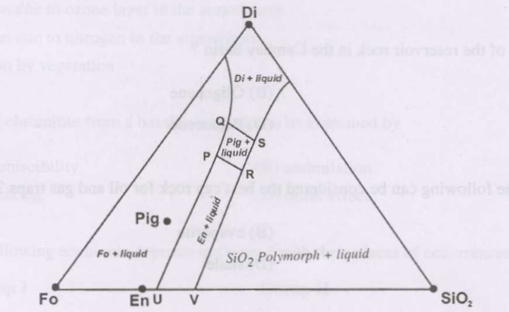
\includegraphics[width=0.5\columnwidth]{figs/IMG-1 2009.png}
        \caption{ Questions 51 and 52 }
        \label{fig:placeholder_1}
    \end{figure}
    

    \item The name of the rock is \hfill{\brak{\text{GATE GG 2009}}} 
            \begin {enumerate}
                \begin{multicols}{2}
                    \item Lherzolite
                    \item Harzburgite
                    \item Wehrlite
                    \item Dunite
                \end{multicols}
            \end{enumerate}
    \item On partially melting this rock, the first melt will have the composition of point \hfill{\brak{\text{GATE GG 2009}}} 
            \begin {enumerate}
                \begin{multicols}{2}
                    \item P
                    \item Q
                    \item R
                    \item S
                \end{multicols}
            \end{enumerate}
\subsection*{Common Data Questions 53 and 54: }
    An unfossiliferous sedimentary succession is characterized by the following features - 
    $\brak{i}$ sandstone-shale alternation, with sheet-like geometry of the sandstone beds;$\brak{ii}$ the sandstones exhibit graded bedding;$\brak{iii}$ erosional structures under the sandstone beds;$\brak{iv}$ convolute lamination, and $\brak{v}$ripple marks on the sandstone beds.

    \item Which depositional environment is indicated for the above sedimentary succession? \hfill{\brak{\text{GATE GG 2009}}} 
            \begin {enumerate}
                \begin{multicols}{2}
                    \item Fluvial
                    \item Eolian
                    \item Intertidal
                    \item Deep marine
                \end{multicols}
            \end{enumerate}
    \item What type of paleocurrent pattern is expected from the erosional structures in the succession? \hfill{\brak{\text{GATE GG 2009}}} 
            \begin {enumerate}
                \begin{multicols}{2}
                    \item Unimodal
                    \item Bimodal
                    \item Bimodal - bipolar
                    \item Polymodal
                \end{multicols}
            \end{enumerate}
\subsection*{Common Data Questions 55 and 56: }
    Examine the given geological section, which contains sedimentary successions interrupted by a dyke, and which contains no tectonic discontinuities.

    \begin{figure}[H]
        \centering
        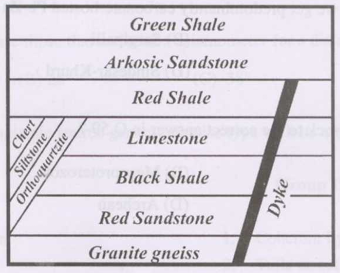
\includegraphics[width=0.5\columnwidth]{figs/IMG-2 2009.png}
        \caption{ Questions 55 and 56 }
        \label{fig:placeholder_2}
    \end{figure}
    
    \item How many unconformities can be identified in the section? \hfill{\brak{\text{GATE GG 2009}}} 
            \begin {enumerate} 
                \begin{multicols}{2}
                    \item $3$
                    \item $4$
                    \item $5$
                    \item $6$
                \end{multicols}
            \end{enumerate}
    \item Which of the following contacts is a nonconformity? \hfill{\brak{\text{GATE GG 2009}}} 
            \begin {enumerate}
                    \item Granite gneiss - Red Sandstone
                    \item Black Shale - Limestone
                    \item Limestone - Red Shale
                    \item Red Shale - Arkosic Sandstone
            \end{enumerate}
\section*{Linked Answer Questions}
\subsection*{Statement for Linked Answer Questions 57 and 58: }

    Microfossils may have following is a siliceous microfossil group ?
    \item Which of the following is a siliceous microfossil group? \hfill{\brak{\text{GATE GG 2009}}} 

            \begin {enumerate}
                \begin{multicols}{2}
                    \item Conodonts
                    \item Radiolaria
                    \item Dinoflagellates
                    \item Foraminifera
                \end{multicols}
            \end{enumerate}
    \item What is the preferred microhabitat of the microfossil group that is the correct answer in Q.57? \hfill{\brak{\text{GATE GG 2009}}} 
            \begin {enumerate}
                \begin{multicols}{2}
                    \item Benthic
                    \item Planktic
                    \item Nektic
                    \item Nektobenthic
                \end{multicols}
            \end{enumerate}
\subsection*{Statement for Linked Answer Questions 59 and 60: }
    $Pb-Zn$ sulphide deposits can form in different types of host rocks.
    \item Of the following, where do we get predominantly carbonate-hosted $Pb-Zn$ sulphide deposits? \hfill{\brak{\text{GATE GG 2009}}} 
            \begin {enumerate}
                \begin{multicols}{2}
                    \item Mochia - Zawar
                    \item Sargipalli
                    \item Pur - Banera
                    \item Sindesar-Khurd
                \end{multicols}
            \end{enumerate}
    \item What is the age of the host rock to the correct answer in $Q.59$? \hfill{\brak{\text{GATE GG 2009}}} 
            \begin {enumerate}
                \begin{multicols}{2}
                    \item Neoproterozoic
                    \item Mesoproterozoic
                    \item Paleoproterozoic
                    \item Archean
                \end{multicols}
            \end{enumerate}
    \centerline{\textbf{END OF SECTION 1 OF PART B }}
    \begin{center}
        \subsection*{PART B (SECTION 2): FOR GEOPHYSICS CANDIDATES ONLY}
    \end{center}
 
 \end{enumerate}
\subsubsection*{Q.20 - Q.60 carry two marks each.}
\begin{enumerate}[start = 21]
    \item Match the following functions in time-domain with their Fourier spectra: \hfill{\brak{\text{GATE GG 2009}}} 
            \begin{multicols}{2}
                \hspace{4em}{\textbf{Group $I$}}
                \begin{enumerate}[start=16]
                            \item $\Pi{(t)} =
                                        \begin{cases}
                                        1,-1/2\leq t \leq 1/2\\
                                        0,t<-1/2\text{ and }\hspace{.25cm}t>1/2
                                        \end{cases}  $    
                            \item Dirac delta function, $\delta(t)$
                            \item $x(t) = e^{-\mydet{t}}$
                            \item $\Lambda{(t)} =
                                    \begin{cases}
                                    1+t,-1<t<0\\
                                    1-t,0<t<1\\
                                    0,\text{otherwise}
                                    \end{cases}  $
                \end{enumerate}
                
    
                \columnbreak
                
                \hspace{5em}{\textbf{Group $II$}} 
                \begin{enumerate}            
                    \item $1$ 
                    \item $ \frac{\sin{\brak{\pi f}}}{f} \text{,where f is frequency }$
                    \item $ \frac{2}{1+4\pi^2f^2}\text{,where f is frequency }$
                    \item $ \frac{\sin^2\brak{\pi f}}{f^2}\text{,where f is    frequency }$
                \end{enumerate}
               
            \end{multicols}
                \begin {enumerate}
                    \begin{multicols}{2}
                        \item P-$2$, Q-$3$, R-$1$, S-$4$
                        \item P-$1$, Q-$3$, R-$2$, S-$4$
                        \item P-$1$, Q-$4$, R-$2$, S-$3$
                        \item P-$2$, Q-$1$, R-$3$, S-$4$
                    \end{multicols}
                \end{enumerate}
    \item The teleseismic rays are those that arrive at a seismometer for a distance greater than \hfill{\brak{\text{GATE GG 2009}}} 
            \begin {enumerate}
                \begin{multicols}{4}
                    \item $18\degree$
                    \item $28\degree$
                    \item $38\degree$
                    \item $48\degree$
                \end{multicols}
            \end{enumerate}
    \item Match the following seismic source generated noise type with its appearance on the seismogram : \hfill{\brak{\text{GATE GG 2009}}} 
                    
            \begin{multicols}{2}           
            \hspace{2em}{\textbf{Group $I$}}
            \begin{enumerate}[start=16]
                \item Reverberation
                \item Multiples
                \item Guided waves
                \item Diffractions
            \end{enumerate}
            
            \columnbreak
            
            \hspace{2em}{\textbf{Group $II$}}
            \begin{enumerate} 
                \item Coherent hyperbolic events
                \item Tails on reflected events
                \item Events paralleling first breaks
                \item Reflections at even time intervals after the primary reflections
            \end{enumerate}                       

        \end{multicols}
            \begin {enumerate}
                \begin{multicols}{2}
                    \item P-$1$, Q-$3$, R-$2$, S-$4$
                    \item P-$3$, Q-$4$, R-$2$, S-$1$
                    \item P-$2$, Q-$4$, R-$3$, S-$1$
                    \item P-$4$, Q-$1$, R-$3$, S-$2$
                \end{multicols}
            \end{enumerate}
    \item Which is the parameter for measuring the size of the earthquake that does not need an instrumental record? \hfill{\brak{\text{GATE GG 2009}}} 
            \begin {enumerate}
                \begin{multicols}{2}
                    \item Richter Magnitude
                    \item Intensity
                    \item Moment
                    \item M$_W$
                \end{multicols}
            \end{enumerate}  
    \item The standard form of wave equation for propagation of cubical dilatation $\brak{\theta}$ is \hfill{\brak{\text{GATE GG 2009}}} 
    $$\rho\frac{\partial^2\theta}{\partial t^2} = \brak{\lambda + 2\mu }\nabla^2\theta$$
    The compressional wave velocity is given by 
   
    
            \begin {enumerate}
                \begin{multicols}{4}
                    \item $\sqrt{\frac{2\lambda + \mu }{\rho}}$
                    \item $\sqrt{\frac{\lambda + 2\mu }{2\rho}}$
                    \item $\sqrt{\frac{\lambda + \mu }{\rho}}$
                    \item $\sqrt{\frac{\lambda + 2\mu }{\rho}}$
                \end{multicols}
            \end{enumerate}

    \item PKIKP is a seismic body wave which travels through \hfill{\brak{\text{GATE GG 2009}}} 
            \begin{enumerate}
                \item upper mantle
                \item upper and lower mantle
                \item mantle, outer core and inner core
                \item mantle and outer core                
            \end{enumerate}
    \item A seismic signal is recorded in a frequency band, $50-100\,Hz$. The sampling interval $\brak{ms}$ to avoid aliasing would be \hfill{\brak{\text{GATE GG 2009}}} 
            \begin {enumerate}
                \begin{multicols}{4}
                    \item $5$
                    \item $10$
                    \item $15$
                    \item $20$
                \end{multicols}
            \end{enumerate}
    \item The minimum appreciable amplitude recorded by a seismometer is $0.2\,mm$ and the maximum one is $20.0\,cm$, then the dynamic range in $dB$ is \hfill{\brak{\text{GATE GG 2009}}} 
            \begin {enumerate}
                \begin{multicols}{4}
                    \item $80$
                    \item $60$
                    \item $40$
                    \item $20$
                \end{multicols}
            \end{enumerate}
    \item Match the following: \hfill{\brak{\text{GATE GG 2009}}} 
                    
            \begin{multicols}{2}
            \hspace{2em}{\textbf{Group $I$}}
            
            \begin{enumerate}[start=16]
                \item Primary wave
                \item Secondary wave
                \item Rayleigh wave
                \item Love wave
            \end{enumerate}

            \columnbreak
            
            \hspace{2em}{\textbf{Group $II$}}
            
            \begin{enumerate} 
                \item Propagate along surface of the medium
                \item Particle motion is orthogonal to direction of propagation
                \item Particle motion describes a retrograde ellipse
                \item Particle motion in the direction of propagation
            \end{enumerate}
        \end{multicols}
            \begin {enumerate}
                \begin{multicols}{2}
                    \item P-$3$, Q-$4$, R-$1$, S-$2$
                    \item P-$1$, Q-$4$, R-$2$, S-$3$
                    \item P-$1$, Q-$3$, R-$2$, S-$4$
                    \item P-$4$, Q-$2$, R-$3$, S-$1$
                \end{multicols}
            \end{enumerate}
    
    \item  Which of the following is a minimum-phase wavelet? The first value in each case is at time zero. \hfill{\brak{\text{GATE GG 2009}}} 
            \begin {enumerate}
                \begin{multicols}{2}
                    \item $\cbrak{-2,5,-2}$
                    \item $\cbrak{-2,5,2}$
                    \item $\cbrak{6,-1,-2}$
                    \item $\cbrak{3,4,-4}$
                \end{multicols}
            \end{enumerate}
    \item In a gas zone, true porosity $\phi_t$, neutron $\log{\phi_n}$, and density derived porosity $\phi_d$are related as \hfill{\brak{\text{GATE GG 2009}}} 
            \begin {enumerate}
                \begin{multicols}{2}
                    \item $\phi_n<\phi_d>\phi_t$
                    \item $\phi_n>\phi_d>\phi_t$
                    \item $\phi_n>\phi_d=\phi_t$
                    \item $\phi_n<\phi_d=\phi_t$
                \end{multicols}
            \end{enumerate}
    \item Identify the equation for formation water resistivity $\brak{Rw_e}$ estimation from SP log, wherein $SSP$, $K\brak{T}$, and $R_{mfe}$ are respectively static SP, temperature dependent coefficient and mudfiltrate resistivity . \hfill{\brak{\text{GATE GG 2009}}} 
            
            \begin{enumerate}
                \item $\hspace{.25cm}SSP=-Rw_e\log{\brak{\frac{K\brak{T}}{R_{mfe}}}}$
                \item $\hspace{.25cm}SSP=-K\brak{T}\log{\brak{\frac{Rw_e}{R_{mfe}}}}$
                \item $\hspace{.25cm}SSP=-R_{mfe}\log{\brak{\frac{K\brak{T}}{Rw_e}}}$
                \item $\hspace{.25cm}SSP=-K\brak{T}\log{\brak{\frac{R_{mfe}}{Rw_e}}}$
            \end{enumerate}
            
    \item Gamma ray detected in density log is \hfill{\brak{\text{GATE GG 2009}}} 
            \begin{enumerate}
                \item natural gamma present in the formation
                \item gamma ray from epithermal neutron source
                \item gamma ray scattered from the formation
                \item gamma ray emitted from neutron capture reaction               
            \end{enumerate}
    \item In Turam method, one measures the reduced field ratio of the amplitude and of the phase difference between the two coils. In the absence of subsurface conducting body, the response is characterized as \hfill{\brak{\text{GATE GG 2009}}} 
            \begin{enumerate}
                \item the successive reduced field ratio is equal to 1.0 and phase difference is $0\degree$
                \item the successive reduced field ratio is equal to 1.0 and phase difference is $45\degree$ 
                \item the successive reduced field ratio is equal to 0.5 and phase difference is $90\degree$
                \item the successive reduced field ratio is equal to 0.5 and phase difference is $60\degree$                
            \end{enumerate}
    \item  Electric field \brak{\overrightarrow{E}} through a polarizable dielectric medium with polarization vector \brak{\overrightarrow{P}}, electric susceptibility $\brak{\chi_e}$ and dielectric permittivity \brak{\varepsilon_0}. The electric displacement vector \brak{\overrightarrow{D}} for the medium can be written as \hfill{\brak{\text{GATE GG 2009}}} 
            \begin {enumerate}
                \begin{multicols}{2}
                    \item $\overrightarrow{D} = \varepsilon_0\brak{1 + \chi_e} $
                    \item $\overrightarrow{D} = \varepsilon_0\overrightarrow{E} - \overrightarrow{P}$
                    \item $\overrightarrow{D} = \varepsilon_0\overrightarrow{E} + \chi_e$
                    \item $\overrightarrow{D}= \varepsilon_0\overrightarrow{E} + \overrightarrow{P}$
                \end{multicols}
            \end{enumerate}
    \item Using different electrodes configuration, maximum depth of investigation is achieved in \hfill{\brak{\text{GATE GG 2009}}} 
            \begin {enumerate}
                \begin{multicols}{2}
                    \item Schlumberger
                    \item dipole
                    \item tri-electrodes
                    \item Wenner
                \end{multicols}
            \end{enumerate}
    \item Relevant differential equation to study low frequency electromagnetic prospecting for a conducting target can be written in the form of \hfill{\brak{\text{GATE GG 2009}}} 
            \begin {enumerate}
                \begin{multicols}{2}
                    \item Wave equation
                    \item Laplace's equation
                    \item Helmholtz equation
                    \item Poisson's equation
                \end{multicols}
            \end{enumerate}
    \item In a layered medium, if the basement is perfectly conducting, magnetotelluric phase response asymptotically approaches to \hfill{\brak{\text{GATE GG 2009}}} 
            \begin {enumerate}
                \begin{multicols}{2}
                    \item $0\degree$
                    \item $45\degree$
                    \item $60\degree$
                    \item $90\degree$
                \end{multicols}
            \end{enumerate}
    \item Magnetotelluric spectral impedance can be defined as \hfill{\brak{\text{GATE GG 2009}}} 
            \begin{enumerate}
                \item the ratio of the spatial spectrum from mutually orthogonal horizontal components of the electric and magnetic field
                \item the ratio of the spatial spectrum of the vertical component to the horizontal component of magnetic field
                \item the ratio of the spatial spectrum of the vertical component to the horizontal component of electric magnetic field
                \item the ratio of the spatial spectrum of the two horizontal components of electric field                 
            \end{enumerate}
    \item Following four electrodes array: P1, P2 are measuring electrodes and C1, C2 are current electrodes used in resistivity measurement. Inter-electrode separation is also shown in figure.\hfill{\brak{\text{GATE GG 2009}}} 
    \begin{figure}[H]
        \centering
        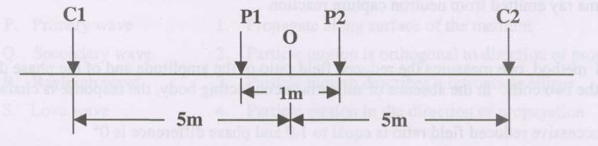
\includegraphics[width=1\columnwidth]{figs/IMG-3_2009.png}
        \caption{Q.40.}
        \label{fig:placeholder}
    \end{figure}
   
    The above electrodes configuration is 
    \begin{enumerate}
        \begin{multicols}{2}
            \item radial dipole
            \item parallel dipole
            \item Schlumberger 
            \item Wenner
        \end{multicols}
    \end{enumerate}
     \item In DC resistivity method, direct filter coefficients are used to compute \hfill{\brak{\text{GATE GG 2009}}} 
            \begin{enumerate}
                \item apparent resistivity data from resistivity transform
                \item resistivity transform from apparent resistivity data
                \item apparent resistivity from measured potential difference
                \item apparent resistivity from one electrode configuration to other electrode configuration                
            \end{enumerate}
    \item A counting rate of $15,100$ counts per minute is recorded by a radiation counter having a dead time of $300\,\mu sec$. The count rate (counts per minute) in the absence of dead time \hfill{\brak{\text{GATE GG 2009}}} 
            \begin {enumerate}
                \begin{multicols}{4}
                    \item $13,333$
                    \item $14,333$
                    \item $15,333$
                    \item $16,333$
                \end{multicols}
            \end{enumerate}
     \item The output of a linear and invariant system for a unit input is $\cbrak{3,1}$. Then what would be the output for an input $\cbrak{-2,1}$? \hfill{\brak{\text{GATE GG 2009}}} 
            \begin {enumerate}
                \begin{multicols}{4}
                    \item $\cbrak{-6,1,1}$
                    \item $\cbrak{-1,1,6}$
                    \item $\cbrak{-1,6,1}$
                    \item $\cbrak{1,-1,6}$
                \end{multicols}
            \end{enumerate}
    \item Geophysical inverse problems are described by \hfill{\brak{\text{GATE GG 2009}}} 
            \begin{enumerate}
                \item Fredholm's integral equation of first kind
                \item Fredholm's integral equation of second kind
                \item Volterra's equation of second kind
                \item Legendre equation                
            \end{enumerate}
    \item Spot the ANN method from the following: \hfill{\brak{\text{GATE GG 2009}}} 
            \begin{enumerate}
                \item Singular value decomposition
                \item Monte-Carlo technique
                \item Ridge regression procedure
                \item Back propagation technique                
            \end{enumerate}
    \item The concept of resolving kernel is used in \hfill{\brak{\text{GATE GG 2009}}} 
            \begin{enumerate}
                \item Tikhonov's regularization method
                \item Ridge regression method
                \item Backus-Gilbert method
                \item Simulated annealing method                
            \end{enumerate}
    \item For underwater gravity measurements, the following correction is needed: \hfill{\brak{\text{GATE GG 2009}}} 
            \begin{enumerate}
                \item Prey correction
                \item Free-air correction
                \item Bouguer correction
                \item Isostatic correction                
            \end{enumerate}
    \item The source of magnetic anomalies extend up to \hfill{\brak{\text{GATE GG 2009}}} 
            \begin{enumerate}
                \item upper mantle
                \item core-mantle boundary
                \item lower mantle
                \item Curie-point isotherm                
            \end{enumerate}
    \item In magnetic prospecting scalar magnetometers are used. Then, the prime assumption involved in magnetic data acquisition is \hfill{\brak{\text{GATE GG 2009}}} 
            \begin{enumerate}
                \item remnant magnetization is predominant
                \item both remnant and induced magnetization are responsible
                \item induced magnetization plays a dominant role
                \item only diamagnetic sources are responsible                 
            \end{enumerate}
    \item Source of main geomagnetic field is best represented by \hfill{\brak{\text{GATE GG 2009}}} 
            \begin{enumerate}
                \item a system of electric currents at core-mantle boundary
                \item a system of dipoles, quadrupoles, octupoles and multipoles
                \item an inclined geomagnetic dipole at center of earth
                \item a system of currents in the ionosphere                
            \end{enumerate}
\section*{Common Data Questions}
\subsection*{Common Data Questions 51 and 52: }
    In a resistivity sounding experiment using Schlumberger configuration the apparent resistivity function asymptotically approaches a sloping straight line of slope $45\degree$ with abscissa.
        \item From the above data it can be inferred that the basement is \hfill{\brak{\text{GATE GG 2009}}} 
                \begin {enumerate}
                    \begin{multicols}{2}
                        \item Perfectly conducting
                        \item Relatively resistive
                        \item Relatively conducting
                        \item Perfectly resistive
                    \end{multicols}
                \end{enumerate}
    \item If the intercept at $\rho_a = 1\,ohm-m$ is 5 and resistivity of top layer is $10\,ohm-m$ , then the depth of basement is \hfill{\brak{\text{GATE GG 2009}}} 
            \begin {enumerate}
                \begin{multicols}{2}
                    \item $50.0\,m$
                    \item $5.0\,m$
                    \item $2.0\,m$
                    \item $0.5\,m$
                \end{multicols}
            \end{enumerate}
\subsection*{Common Data Questions 53 and 54: }
    In a seismic refraction experiment involving a two-layered earth of P-wave velocities, $3\,km/sec$ and $4.5\,km/sec$ the delay time is found to be $49.69\, ms$.
        \item From the above data, the depth to the interface is given by \hfill{\brak{\text{GATE GG 2009}}} 
                \begin {enumerate}
                    \begin{multicols}{2}
                        \item $150\,m$
                        \item $120\,m$
                        \item $100\,m$
                        \item $50\,m$
                    \end{multicols}
                \end{enumerate}
    \item Using the above depth, the computed critical distance $\brak{m}$ would be \hfill{\brak{\text{GATE GG 2009}}} 
            \begin {enumerate}
                \begin{multicols}{2}
                    \item $151.20$
                    \item $178.88$
                    \item $221.67$
                    \item $169.87$
                \end{multicols}
            \end{enumerate}
\subsection*{Common Data Questions 55 and 56: }
    The peak gravity anomaly over a 2-D line mass of circular cross-section \brak{horizontal cylinder} of density contrast $500\,kg/m^3$ is $1.674\,mgal$. The anomaly decreases to $0.837\,mgal$ at a distance of $500\,m$ along a principal profile. The universal gravitation constant, $G = 6.6667\times10^{-11}m^3sec^{-2}kg^{-1}$
        \item The depth $\brak{m}$ to center of line mass and radius $\brak{m}$ of the horizontal cylinder are \hfill{\brak{\text{GATE GG 2009}}} 
                \begin {enumerate}
                    \begin{multicols}{2}
                        \item $500$, $199.80$
                        \item $200$, $150.93$
                        \item $200$, $100.33$
                        \item $100$, $60.37$
                    \end{multicols}
                \end{enumerate}
    \item Hence compute the excess mass per unit length $\brak{kg/m}$ of the line mass \hfill{\brak{\text{GATE GG 2009}}}
            \begin {enumerate}
                \begin{multicols}{2}
                    \item $11.0 \times 10^7$
                    \item $9.0 \times 10^7$
                    \item $6.27 \times 10^7$
                    \item $3.67 \times 10^7$
                \end{multicols}
            \end{enumerate}
\section*{Linked Answer Questions}
\subsection*{Statement for Linked Answer Questions 57 and 58: }
    Resistivity log recorded using normal device with measuring electrode, $M$, is situated close to the current electrode, $A$, in logging device placed in borehole. A constant current, $I$, injected from current electrode into the formation.
        \item If the spacing between $A$ and $M$ is $r$, and the potential difference $\Delta V$ is measured between the measuring electrode, $M$ and remotely placed surface electrode. Then the expression for the apparent resistivity can be written as \hfill{\brak{\text{GATE GG 2009}}} 
                    \begin{enumerate}
                        \begin{multicols}{2}
                            \item$ \rho_a = \frac{2\pi r}{I}\Delta V$
                            \item$ \rho_a = \frac{4\pi r^2 }{I}\Delta V $
                            \item$ \rho_a = \frac{2\pi r^2}{I}\Delta V$
                            \item$ \rho_a = \frac{4\pi r }{I}\Delta V $
                        \end{multicols}
                    \end{enumerate}
    \item If $r = 0.40\,m$ ; $I = 0.02\,amp$ ; $\Delta V =0.04\,volt$, then the measured apparent resistivity will be \hfill{\brak{\text{GATE GG 2009}}} 
            \begin {enumerate}
                \begin{multicols}{2}
                    \item $1\,\Omega m$
                    \item $5\,\Omega m$
                    \item $10\,\Omega m$
                    \item $20\,\Omega m$
                \end{multicols}
            \end{enumerate}
\subsection*{Statement for Linked Answer Questions 59 and 60: }
    Given the wavelets,$a=\cbrak{3,-2} \text{ and } b = \cbrak{1,-2}$
        \item The cross-correlation, $\phi_{ab}$, is given by \hfill{\brak{\text{GATE GG 2009}}} 
            \begin{enumerate}
                \begin{multicols}{2}
                    \item $\cbrak{-6,7,-2}$
                    \item $\cbrak{-6,10,-12}$
                    \item $\cbrak{-4,-11,-6}$
                    \item $\cbrak{-6,11,-4}$
                \end{multicols}            
            \end{enumerate}
    \item The inverse of wavelet $a$,$W^{-1}_a$ is given by \hfill{\brak{\text{GATE GG 2009}}} 
        \begin{enumerate}
            \begin{multicols}{2}
                \item $\cbrak{4/3, 16/9, 17/7, 64/81}$
                \item $\cbrak{1/3, 2/9, 4/27, 8/81}$
                \item $\cbrak{4/9, 1/3, 64/81, 16/27}$
                \item $\cbrak{16/27, 64/81, 4/9, 1/3}$
            \end{multicols}

        \end{enumerate}
    \centerline{\textbf{END OF THE QUESTION PAPER}}
 \end{enumerate}
\end{document}
